% This is samplepaper.tex, a sample chapter demonstrating the
% LLNCS macro package for Springer Computer Science proceedings;
% Version 2.21 of 2022/01/12
%
\documentclass[runningheads]{llncs}
%
\usepackage[T1]{fontenc}
% T1 fonts will be used to generate the final print and online PDFs,
% so please use T1 fonts in your manuscript whenever possible.
% Other font encondings may result in incorrect characters.
%
\usepackage{graphicx}
% Used for displaying a sample figure. If possible, figure files should
% be included in EPS format.
%
% If you use the hyperref package, please uncomment the following two lines
% to display URLs in blue roman font according to Springer's eBook style:
%\usepackage{color}
%\renewcommand\UrlFont{\color{blue}\rmfamily}
%\urlstyle{rm}
%
% Ajusta el espacio que LaTeX deja entre los bloques flotantes (como las figuras) y el texto normal
\setlength{\textfloatsep}{10pt}    % Por defecto suele ser20pt
\setlength{\intextsep}{10pt}         % Espacio arriba/abajo de una figura "aquí" [h]
\usepackage{booktabs}
\begin{document}
%
\title{Modulo 3: Simulacion por eventos discretos}
%
%\titlerunning{Abbreviated paper title}
% If the paper title is too long for the running head, you can set
% an abbreviated paper title here
%
\author{Los Tecnicos\\ Rocío Alarcón \and
Ignacio Coronado\and
Maite Aquilar\\
Franca Bielsa\and Camila Sotelo}
%
\authorrunning{F. Author et al.}
% First names are abbreviated in the running head.
% If there are more than two authors, 'et al.' is used.
%
\institute{Universidad nacional de cuyo, Facultad de ingeniería POBOX 5502 \url{http://ingeniería.uncuyo.edu.ar} \and Tecnicas y Herramientas Modernas 2026 }  
%
\maketitle              % typeset the header of the contribution
%
\begin{abstract}
En el siguiente informe se hablará acerca de el programa de Simulación llamado Simul8. Durante las clases se introducieron los conceptos básicos del software, explicando cada uno 
de los elementos que lo componen y las funciones principales de éstos. Como cierre del módulo, se utilizó el software en la resolución de un caso práctico asociado a un proceso productivo seleccionado, acompañado de un análisis financiero.

\keywords{Eventos discretos  \and Simulación \and Simul8 \and Software \and procesos  \and interfaz  \and ingeniería.}
\end{abstract}
%
%
%
\section{Introducción a Simul8}
Se trata de un software de simulación de eventos discretos diseñado para modelar y analizar procesos en diversos sectores como manufactura, logistica, atención médica y servicios. Su interfaz intuitiva de arrastrar y soltar permite a los usuarios construir modelos visuales de sistemas complejos sin necesidad de conocimientos avanzados en programación. También ofrece capacidades avanzadas como la integración de minería de procesos y aprendizaje automático, lo que permite a las organizaciones experimentar con cambios en sus procesos y tomar decisiones informadas sin riesgos, optimizando asi la eficiencia y reduciendo costos.
%
%
%

\subsection{Interfaz del programa}
\begin{figure}[htbp]
    \centering
    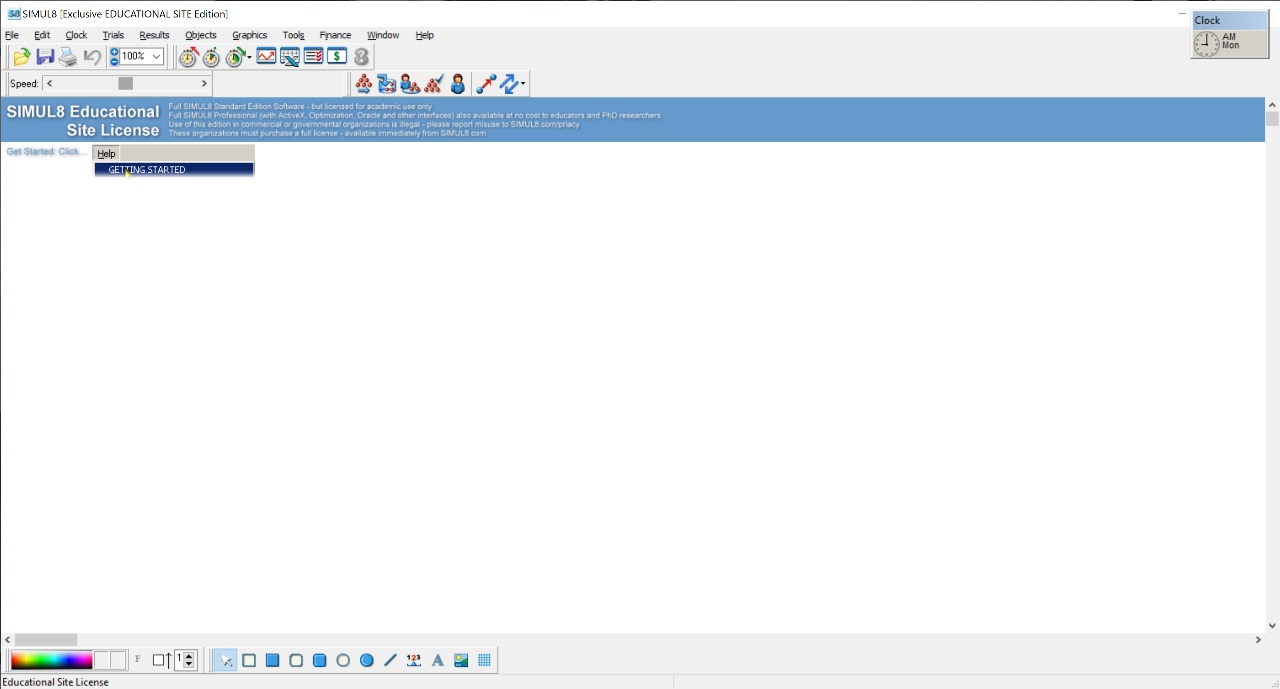
\includegraphics[width=0.5\textwidth]{simul8} 
    \caption{Descripción de la imagen.}
    \label{fig:simul8}
\end{figure}


\section{¿En Qué Consiste SIMUL8?}
El núcleo de SIMUL8 es la construcción de un modelo que imita un proceso real. Este modelo se compone de ``objetos'' que representan las diferentes etapas del proceso[cite: 296]. Los elementos de trabajo (como productos, clientes o documentos) fluyen a través de estos objetos. Al ejecutar la simulación, es posible observar el comportamiento del sistema a lo largo del tiempo, identificar cuellos de botella, medir la utilización de recursos y evaluar el rendimiento general.

Las principales capacidades de SIMUL8 incluyen:
\begin{itemize}
    \item \textbf{Modelado Visual:} Permite construir el diagrama del proceso de forma intuitiva, arrastrando y soltando objetos en la ventana de simulación.
    \item \textbf{Análisis Estadístico:} Incorpora la variabilidad del mundo real mediante distribuciones de probabilidad para tiempos de proceso, llegadas de elementos, etc.
    \item \textbf{Optimización de Recursos:} Ayuda a determinar la cantidad óptima de personal, máquinas o cualquier otro recurso necesario para cumplir con los objetivos.
    \item \textbf{Análisis de Resultados:} Genera reportes detallados y gráficos sobre el rendimiento del sistema, como tiempos de espera, costos, producción y utilización de recursos.
    \item \textbf{Pruebas de Escenarios:} Facilita la comparación de diferentes configuraciones del proceso (``what-if'') para encontrar la solución más eficiente.
\end{itemize}

\section{Significado de los Símbolos en la Barra de Herramientas}
La barra de herramientas de la versión clásica de SIMUL8, como la que se muestra en la imagen siguiente, contiene accesos directos a funciones comunes y a los objetos de simulación principales. Se divide en varias secciones.
\begin{figure}
    \centering
    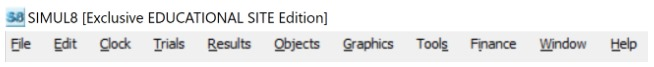
\includegraphics[width=0.9\linewidth]{Barra de Herramientas.jpg}
    \caption{Descripción de la imagen}
    \label{fig:placeholder}
\end{figure}

\noindent Esta es la barra de menú estándar que ofrece acceso a todas las funcionalidades del software, organizadas en categorías:
\begin{description}
    \item[File:] Contiene opciones para crear, abrir, guardar e imprimir simulaciones.
    \item[Edit:] Ofrece herramientas para cortar, copiar, pegar y deshacer acciones.
    \item[Clock:] Permite configurar el tiempo de la simulación (duración, unidades, calentamiento).
    \item[Trials:] Se usa para ejecutar múltiples réplicas de la simulación y obtener resultados estadísticamente válidos.
    \item[Results:] Da acceso a los reportes y al gestor de resultados.
    \item[Objects:] Permite crear y gestionar los objetos de la simulación.
    \item[Graphics:] Contiene herramientas para personalizar la apariencia visual de los modelos.
    \item[Tools:] Ofrece utilidades adicionales como el editor de Visual Logic.
    \item[Finance:] Permite incorporar análisis de costos en el modelo.
    \item[Window \& Help:] Gestiona las ventanas de la interfaz y proporciona acceso a la ayuda.
\end{description}

\section{Símbolos de la Barra de Herramientas Principal}
La siguiente barra agrupa funciones para la gestión de archivos, la ejecución del modelo y el acceso a los resultados.
\begin{figure}
    \centering
    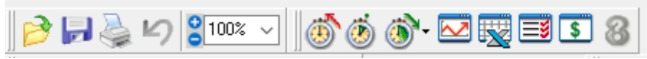
\includegraphics[width=0.8\linewidth]{botones.jpg}
    \caption{Descripción de la imagen}
    \label{fig:placeholder}
\end{figure}


\subsection{Gestión de archivos y vistas}
\begin{itemize}
    \item \textbf{Open (abrir):} Se usa para buscar y abrir un archivo de simulación que ya ha sido guardado en tu computadora.
    \item \textbf{Save (guardar):} Guarda el estado actual de la simulación que tienes abierta. Es crucial para no perder tu trabajo.
    \item \textbf{Print (imprimir):} Permite imprimir una vista del modelo o los reportes de resultados en papel.
    \item \textbf{Undo (deshacer):} Revierte la última acción que realizaste, como mover un objeto o cambiar una configuración.
    \item \textbf{Zoom:} Controla el nivel de acercamiento de la vista del modelo. El 100\% indica la vista normal, y las lupas con + y - permiten acercar o alejar la vista para ver más detalles o el modelo completo.
\end{itemize}

\subsection{Control de simulación y resultados}
\begin{itemize}
    \item \textbf{Clock Properties (propiedades del reloj):} Abre la ventana de configuración del tiempo de la simulación. Aquí defines cuánto durará un día de trabajo, la duración total de la simulación y el período de calentamiento.
    \item \textbf{Run/Pause (ejecutar/pausar):} Inicia la simulación para que los elementos comiencen a fluir por el proceso. Una vez iniciada, el mismo botón sirve para pausar momentáneamente.
    \item \textbf{Reset (reiniciar):} Detiene la simulación y la devuelve a su estado inicial (tiempo cero), borrando todas las estadísticas acumuladas para poder correrla de nuevo.
    \item \textbf{Results Manager (Resultados):} Abre el gestor de resultados, donde puedes ver todas las métricas de rendimiento (KPIs) del modelo, como tiempos de espera, utilización de recursos y cantidad de productos terminados.
    \item \textbf{Calendar (Calendario):} Permite definir horarios de trabajo, turnos y días no laborables para los recursos o para todo el sistema, haciendo el modelo más realista.
    \item \textbf{End of Trail (Fin de la Prueba):} Generalmente asociado a la configuración de pruebas o experimentos. Permite definir las condiciones bajo las cuales una réplica de la simulación debe terminar.
    \item \textbf{Finance (Finanzas):} Activa las funciones de análisis financiero. Permite asignar costos a las actividades, recursos e ítems para calcular la rentabilidad del proceso.
    \item \textbf{Help (Ayuda):} Abre el sistema de ayuda del software para consultar dudas sobre su funcionamiento.
\end{itemize}

\section{Controles de Simulación}
Los siguientes íconos controlan la ejecución del modelo.

\begin{figure}
    \centering
    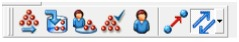
\includegraphics[width=0.8\linewidth]{controles.jpg}
    \caption{Descripción de la imagen.}
    \label{fig:placeholder}
\end{figure}

\noindent En primer lugar, el \textbf{Work Entry Point} (punto de entrada) representa el lugar por el cual ingresan las entidades al sistema. Este elemento permite definir la frecuencia de llegada de las entidades, que puede configurarse de manera determinística o probabilística mediante distribuciones estadísticas[cite: 355]. Por ejemplo, en un modelo de atención al cliente, este punto puede simular la llegada de un cliente cada cierto intervalo de tiempo.

Las \textbf{Work Items} (entidades de trabajo) son las unidades que se desplazan a lo largo del sistema. Estas entidades pueden representar productos, personas, documentos, o cualquier otra unidad de análisis, y pueden portar atributos que afectan su comportamiento dentro del modelo, como prioridades, tipos o tiempos de llegada. Aunque no se representan visualmente de forma independiente, constituyen el núcleo dinámico del sistema modelado.

Las \textbf{Activities} (actividades) corresponden a los procesos que transforman o gestionan las entidades a medida que avanzan en el sistema. Cada actividad puede configurarse con un tiempo de procesamiento específico, el cual puede ser fijo o seguir una distribución de probabilidad. Además, pueden requerir recursos para su ejecución y permiten implementar lógica condicional avanzada. Un ejemplo típico de actividad es el proceso de atención de un cliente o el ensamblaje de una pieza en una línea de producción.

Las \textbf{Queues} (colas) son elementos que permiten modelar la espera de las entidades cuando una actividad está ocupada. Estas colas pueden adoptar distintos criterios de ordenamiento, como FIFO (primero en entrar, primero en salir), LIFO (último en entrar, primero en salir), o sistemas con prioridades. Las colas son esenciales para representar fenómenos de congestión y para analizar tiempos de espera y acumulación de trabajo en proceso.

Los \textbf{Resources} (recursos) representan elementos limitados que son necesarios para la ejecución de ciertas actividades. Estos pueden ser personas, máquinas, vehículos u otros dispositivos que no están disponibles en cantidad ilimitada. En el modelo, los recursos se asignan a actividades específicas y pueden configurarse con restricciones de disponibilidad, como turnos o tiempos de inactividad. Su adecuada gestión es crucial para evaluar la eficiencia del sistema.

El \textbf{Work Exit Point} (punto de salida) indica el lugar por donde las entidades abandonan el sistema una vez que han completado su paso por las actividades modeladas. Este elemento permite cuantificar la salida de productos o servicios y calcular indicadores de rendimiento como el \textit{throughput} (rendimiento del sistema).

Por otro lado, los \textbf{Storage Bins} (almacenes) son espacios de almacenamiento donde las entidades pueden permanecer sin un orden de servicio determinado. A diferencia de las colas, no siguen una lógica de espera estructurada. Se utilizan comúnmente para modelar inventarios o zonas de almacenamiento temporal antes de una expedición o procesamiento posterior.

Las \textbf{Routing Arrows} (flechas de enrutamiento) son los conectores que permiten definir el flujo entre los distintos elementos del modelo. Estas conexiones pueden configurarse con distintas lógicas de enrutamiento: aleatoria, proporcional, condicional o basada en atributos de los \textit{work items}. Esto otorga gran flexibilidad para modelar decisiones operativas, bifurcaciones o rutas alternativas dentro del sistema.

\begin{figure}
    \centering
    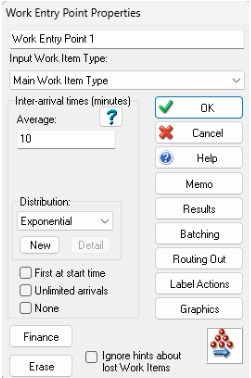
\includegraphics[width=0.4\linewidth]{menu.jpg}
    \caption{Enter Caption}
    \label{fig:placeholder}
\end{figure}

\newpage
\section{Menú desplegable}
Cuando hacemos doble click sobre un centro de trabajo aparece el menú anterior. Posee las siguientes partes:
\begin{itemize}
    \item En la parte superior aparece el casillero en el cuál podemos nombrar al centro de trabajo.
    \item En la pestaña \textbf{Resources} se asignan los recursos que consume el centro de trabajo. Para cada recurso se indica la cantidad máxima y mínima que puede tener el centro de trabajo, así como la distribución de los mismos.
    \item En \textbf{Priority} se indica la prioridad en que van atender los distintos centros de trabajo.
    \item En \textbf{Finance} se indica el costo de capital del centro de trabajo y un costo por unidad o por unidad de tiempo que consume.
    \item En \textbf{Efficiency} se asigna la eficiencia de trabajo del centro de trabajo para atender las entidades de la cola que van llegando.
    \item En \textbf{Routing in} sirve para asignar prioridades o criterios de selección de las entidades o elementos de la cola que serán atendidos primero, es decir que si tenemos múltiples colas que llegan a un centro de trabajo, se asignan con cierto criterio las entidades de las distintas colas que serán seleccionadas.
    \item En \textbf{Routing out} se asigna la prioridad hacia los distintos lugares posibles que pueden ir los elementos o entidades que salen del centro de trabajo según algún criterio, esto serviría cuando el centro de trabajo envíe entidades a distintos lugares.
    \item En \textbf{Distribution} se indica la distribución de probabilidades del tiempo que tarda una entidad (\textit{work item}) en ser procesada por el centro de trabajo. Esta distribución puede obtenerse usando el programa \textbf{StatFit}. En este programa se deberían cargar datos reales de estos tiempos y con ellos se puede estimar la distribución de probabilidad correspondiente. En lo posible conviene una muestra lo suficientemente grande como para que haya una confianza alta en el resultado que ofrece el programa.
\end{itemize}

\section{Matriz de Trabajo}
Simul8 incorpora una herramienta avanzada denominada Matriz de Trabajo (en inglés, \textit{Work Matrix}), que permite modelar con precisión sistemas en los que las entidades poseen comportamientos diferenciados dentro de una misma actividad. Esta funcionalidad es fundamental cuando se desea que un mismo \textit{Work Center} procese distintos tipos de \textit{work items} (entidades) con características operativas propias, como diferentes tiempos de procesamiento, recursos requeridos, o rutas de salida.

La Matriz de Trabajo actúa como una tabla de control que vincula tres dimensiones principales del modelo: el tipo de entidad (identificado mediante un atributo o \textit{label}) y el \textit{Work Center} que la procesa. Esta herramienta permite establecer reglas específicas según el valor de un \textit{label} asignado a las entidades. Por ejemplo, si el \textit{label} \texttt{TipoProducto} distingue entre productos A y B, la Matriz de Trabajo puede definir que:
\begin{itemize}
    \item El Producto A tenga un tiempo de procesamiento fijo de 5 minutos.
    \item Mientras que el Producto B requiera 8 minutos, además de un recurso adicional.
\end{itemize}
De esta manera, se evita la necesidad de duplicar actividades en el modelo y se consigue una representación más compacta y flexible del sistema. El uso de la Matriz de Trabajo es especialmente útil en entornos donde existe variedad de productos, clientes o tareas, como en líneas de producción con múltiples referencias, centros de atención médica con pacientes de distintos niveles de urgencia, o sistemas logísticos con cargas de diferentes características.

\begin{figure}
    \centering
    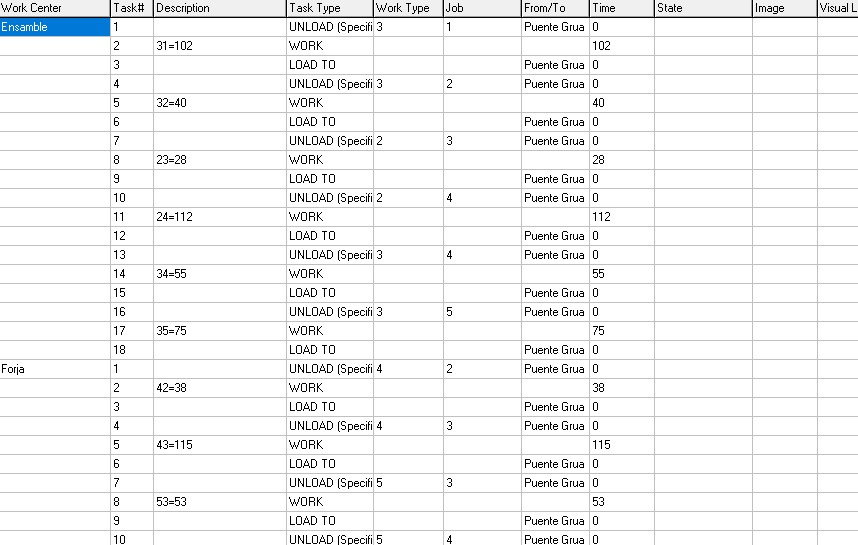
\includegraphics[width=0.9\linewidth]{matriz.jpg}
    \caption{Descripción de la imagen}
    \label{fig:placeholder}
\end{figure}

\newpage
\section{¿Por qué utilizar SIMUL8 y no otras herramientas?}

La selección de una herramienta de simulación de eventos discretos es un factor crítico para el éxito de los proyectos de optimización de procesos en la ingeniería industrial. Si bien el mercado ofrece múltiples alternativas, \textsc{Simul8} se destaca por lograr un equilibrio excepcional entre una curva de aprendizaje sumamente corta y una potencia de cálculo avanzada. A diferencia de las plataformas tradicionales que exigen un dominio profundo de lenguajes de programación complejos, esta herramienta permite a los analistas pasar de la conceptualización de un modelo a la obtención de resultados estadísticos en una fracción del tiempo estimado para otros softwares.

\subsection{Ventajas competitivas de SIMUL8}

\begin{itemize}
    \item \textbf{Velocidad de modelado y prototipado rápido:} Su intuitiva interfaz basada en la filosofía de arrastrar y soltar (\textit{drag-and-drop}) permite estructurar flujos lógicos complejos de forma visual inmediata, acelerando la validación del modelo junto a los dueños del proceso real.
    \item \textbf{Integración nativa con herramientas de análisis de datos:} Permite la vinculación directa con softwares de ajuste de curvas como \textsc{StatFit}, facilitando la conversión de datos históricos de tiempos en distribuciones de probabilidad precisas (exponenciales, normales, \textit{Weibull}, etc.).
    \item \textbf{Simulación de escenarios (``What-if'') y pruebas múltiples:} El gestor de pruebas (\textit{Trials Manager}) posibilita la ejecución automática de múltiples réplicas del modelo bajo diferentes configuraciones de recursos, mitigando la variabilidad estocástica para tomar decisiones respaldadas estadísticamente.
    \item \textbf{Capacidades avanzadas sin código obligatorio:} Elementos como la Matriz de Trabajo (\textit{Work Matrix}) y las lógicas de enrutamiento dinámico permiten modelar sistemas de alta complejidad (con multiplicidad de productos y prioridades) sin necesidad de recurrir a la programación en bloques o código textual.
    \item \textbf{Bajo consumo de recursos computacionales:} A diferencia de los entornos de simulación en 3D inmersivos que demandan hardware gráfico de alta gama, \textsc{Simul8} optimiza la velocidad del motor de cálculo en entornos 2D y 2.5D de forma sumamente ágil.
\end{itemize}



\newpage
\section{Ejemplo práctico:  Elaboración de papel en base a la fibra de caña}
Se ha tomado como referencia una planta ubicada en el Complejo Agroindustrial Ledesma en la provincia de Jujuy 
Se fabrica papel natural bajo la marca Ledesema NAT y es una propuesta íntegramente sustentable, porque son hojas fabricadas con 100\% fibra de caña de azúcar, 0\% fibra de árbol y 0\% blanqueadores químicos.   
\subsection{Descripción del proceso}
En el campo se cosecha, se limpia y se corta la caña de azúcar que irá a los "Trapiches" en donde obtenemos el jugo que utilizamos para producir azúcar y alcohol. De la parte sólida separamos la fibra de la médula.
Luego, la médula se quema en calderas como biomasa para energía y la fibra que se procesa en la planta de celulosa, se utiliza para fabricar pulpa y; con ella, papel.
Para producir 1 tonelada de papel hacen faltan 2 toneladas de fibra de caña de azúcar.
Por otro lado, la planta trabaja en 3 turnos productivos, las 24 horas y los 365 días del año.Con algunas paradas programadas para mantenimiento y limpieza.
La fibra de la caña con la que se produce el papel, es almacenada en una gran pila mediante el denominado "Metodo Ritter"
\subsection {Simulación}
A continuación se presenta un diagrama en donde se simula dicha planta
\begin{figure}
    \centering
    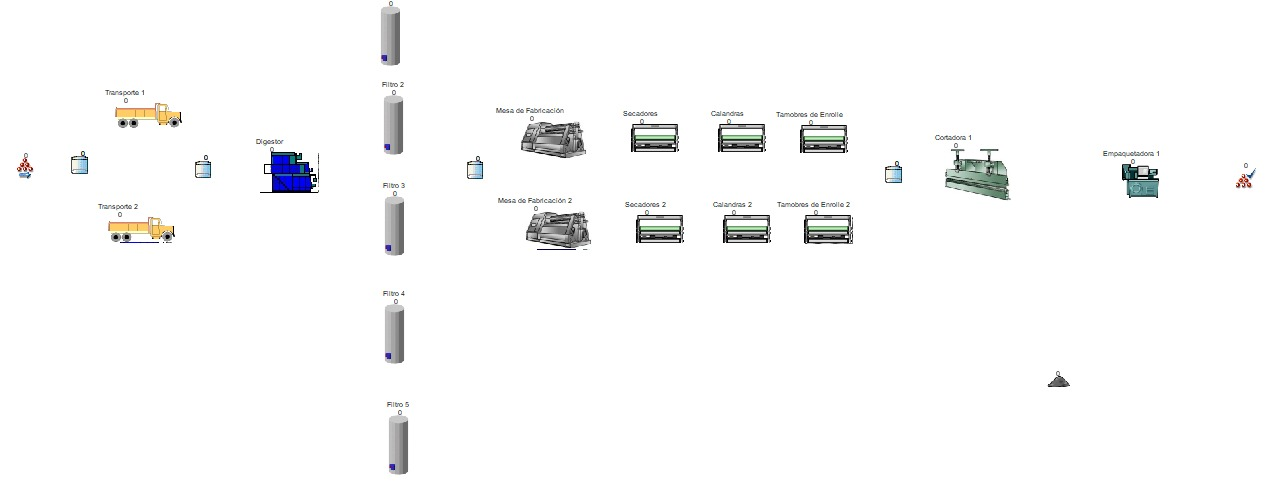
\includegraphics[width=0.9\linewidth]{Circuito en simulacion.jpeg}
    \caption{Circuito en la simulación}
    \label{fig:placeholder}
\end{figure}

¿Cómo funciona?

\noindent Se empieza con la materia prima, en este caso la fibra de caña.
\noindent Luego, la misma será transportada por 2 camiones de gran capacidad.
Como la planta se encuentra al lado de los campos de cultivo de fibra de caña, unicamente se ha considerado el tiempo de carga-descarga de los mismos.
Se ha utilizado 2 camiones para no generar un gran cuello de botella.
A continuación, se sigue por el digestor por donde se cocian en este recipiente junto con químicos y vapor a alta temperatura.
Esto continua por los filtros, en esta parte del proceso si generaría un importante cuello de botella debido a que el tiempo de produccion de los filtros es muy lento con respecto de las otras maquinarias, por lo tanto se han considerado 5 filtros.
Luego, se prosigue con la fabricación de los rollos de papel en la mesa de fabricación. Se han considerado 2 líneas para poder aumentar la producción de la planta y producir rollos de forma más veloz.
Una vez fabricado el rollo, se envían a la cortadora, donde una parte se utiliza para formar hojas de papel y una pequeña parte es residuo.
Finalmente, se empaqueta, dejando la resma lista para su venta y envío.

Cabe destacar que para poder implementarlo en el simulador, se ha tenido que contemplar en el medio de la operación 3 tanques, los cuales representan una posible conversión de unidades
Posteriormente, se contempla cada tanque:

\begin{table}[htbp]
\centering
\caption{Clasificación de los tanques según la etapa del proceso y material.}
\label{tab:procesos_tanques}
% Al poner |l|p{6.5cm}|p{4.5cm}| agregamos los bordes verticales
\begin{tabular}{|l|p{6.5cm}|p{4.5cm}|}
\hline
 & \textbf{Parte del proceso} & \textbf{Unidad} \\
\hline
\textbf{Primer tanque} & Desde la obtención de la materia prima hasta antes del ingreso del digestor & Fibra de caña de azúcar \\
\hline
\textbf{Segundo tanque} & Desde el ingreso de la materia al digestor hasta antes de la mesa de fabricación & Tonelada de papel\\
\hline
\textbf{Tercer tanque} & Desde la mesa de fabricación hasta antes al ingreso a la cortadora & Rollo de papel \\
\hline
\end{tabular}
\end{table}

Sin embargo, el producto final a la venta se considera en toneladas de papel.


\subsection{Análisis Financiero}
En la simulación se consideraron los costos asociados a los siguientes ítems:


1) Costos por Transporte.


2) Salario de los Operarios, siendo 9 en total.


3) Costos por la potencia eléctrica consumida por las maquinarias.


4) Costos del empaquetamiento de las resmas.


\noindent Podemos observar  de nuestra simulación que la ganancia económica es muy grande,  aunque normal en empresas de gran producción de papel como la nuestra la misma no sería realmente representativa ya que se omiten muchos costos asociados a la compra y mantenimiento de las maquinarias, además en una empresa de este calibre hay gran personal trabajando en la parte administrativa de la empresa la cual no se a considerado en esta simulación.

\begin{figure}
    \centering
    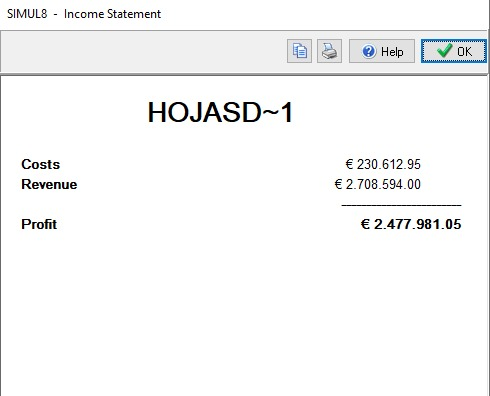
\includegraphics[width=0.7\linewidth]{Finanzas.jpeg}
    \caption{Análisis financiero de la simulación}
    \label{fig:placeholder}
\end{figure}




\newpage
%
% ---- Bibliography ----
%
% BibTeX users should specify bibliography style 'splncs04'.
% References will then be sorted and formatted in the correct style.
%
% \bibliographystyle{splncs04}
% \bibliography{mybibliography}
%
\begin{thebibliography}{8}
\bibitem{ref_article1}
Author, F.: Article title. Journal \textbf{2}(5), 99--110 (2016)

\bibitem{ref_lncs1}
Author, F., Author, S.: Title of a proceedings paper. In: Editor,
F., Editor, S. (eds.) CONFERENCE 2016, LNCS, vol. 9999, pp. 1--13.
Springer, Heidelberg (2016). \doi{10.10007/1234567890}

\bibitem{ref_book1}
Author, F., Author, S., Author, T.: Book title. 2nd edn. Publisher,
Location (1999)

\bibitem{ref_proc1}
Author, A.-B.: Contribution title. In: 9th International Proceedings
on Proceedings, pp. 1--2. Publisher, Location (2010)

\bibitem{ref_url1}
LNCS Homepage, \url{http://www.springer.com/lncs}, last accessed 2023/10/25
\end{thebibliography}
\end{document}
